% !TEX root = Document.tex
%%
%%  Annexes.
%%
%%  Note: Ne pas modifier la ligne ci-dessous.
\addcontentsline{toc}{compteur}{ANNEXES}

\Annexe{Visualisation des étapes de l'algorithme de suivi de mur}
\label{annexe:suivi_mur}
\begin{tabular}{cc}
  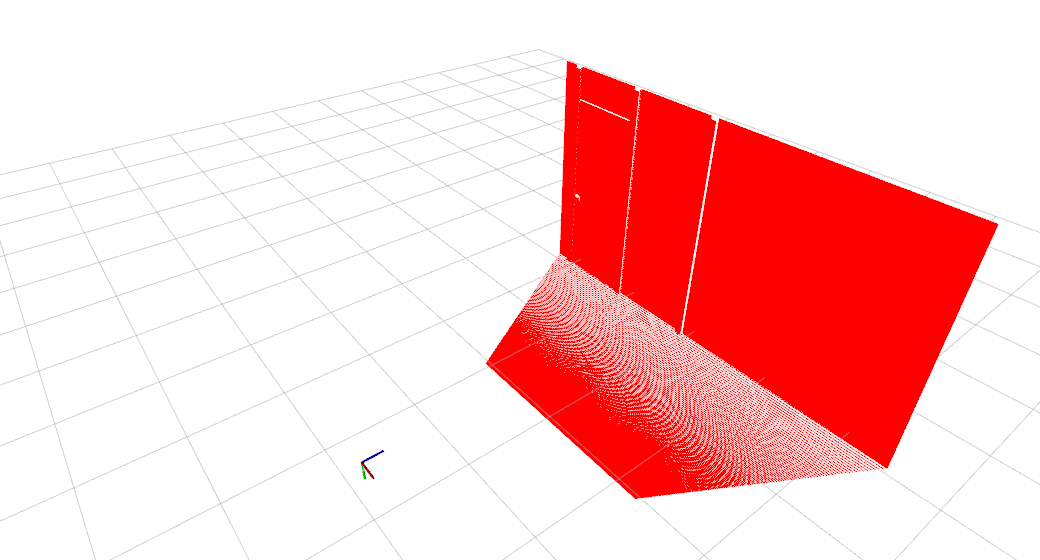
\includegraphics[width=0.5\linewidth]{images/pcl/Selection_060} &
  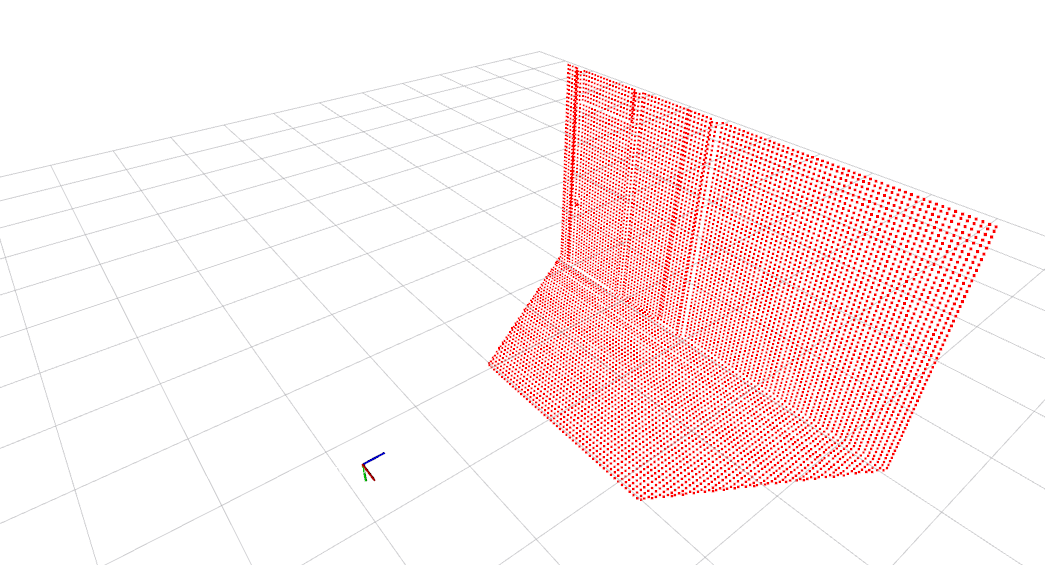
\includegraphics[width=0.5\linewidth]{images/pcl/Selection_061} \\
  (1) & (2) \\
  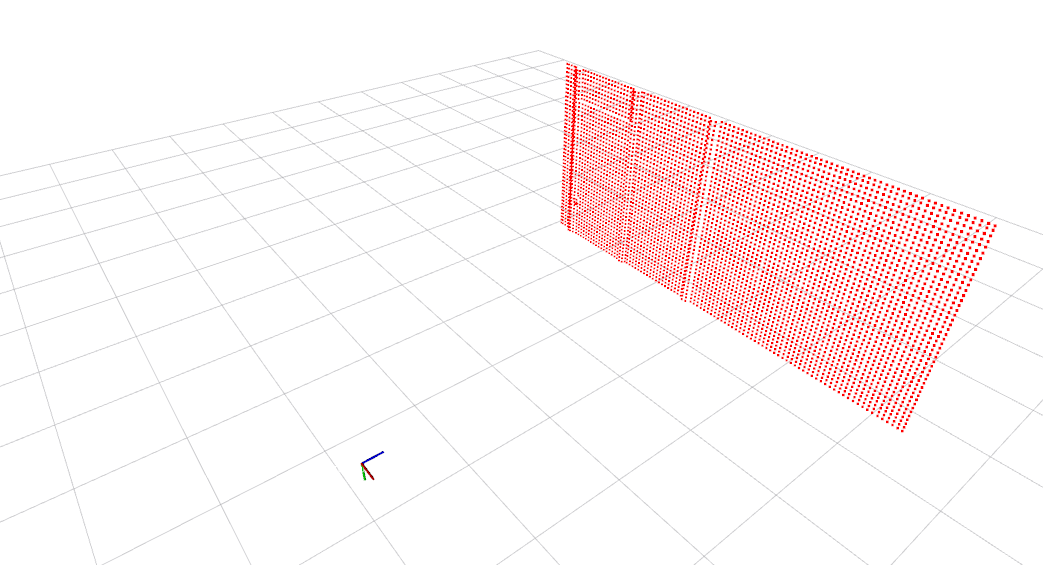
\includegraphics[width=0.5\linewidth]{images/pcl/Selection_062} &
  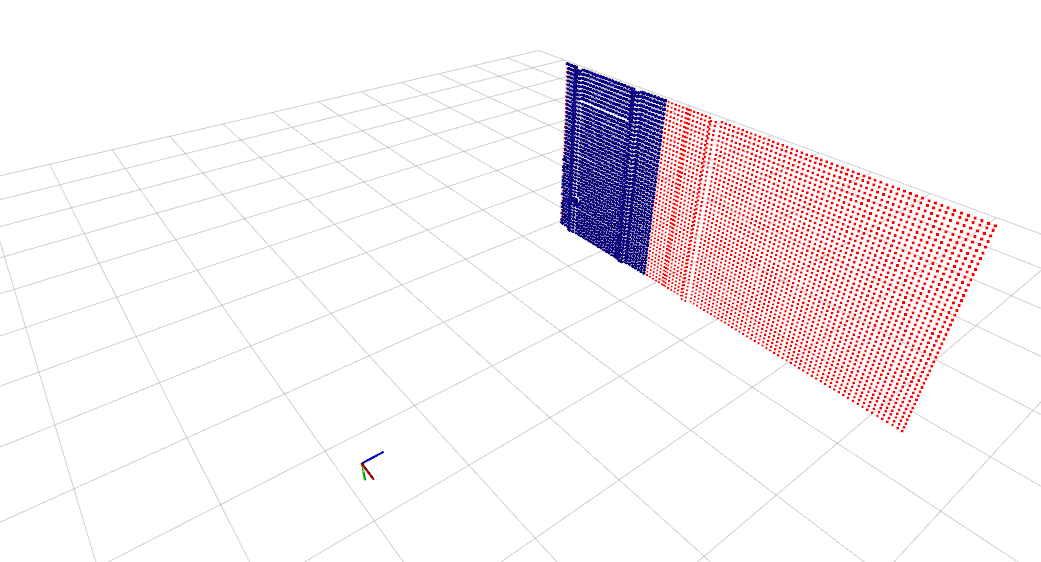
\includegraphics[width=0.5\linewidth]{images/pcl/Selection_063} \\
  (3) & (4) \\
  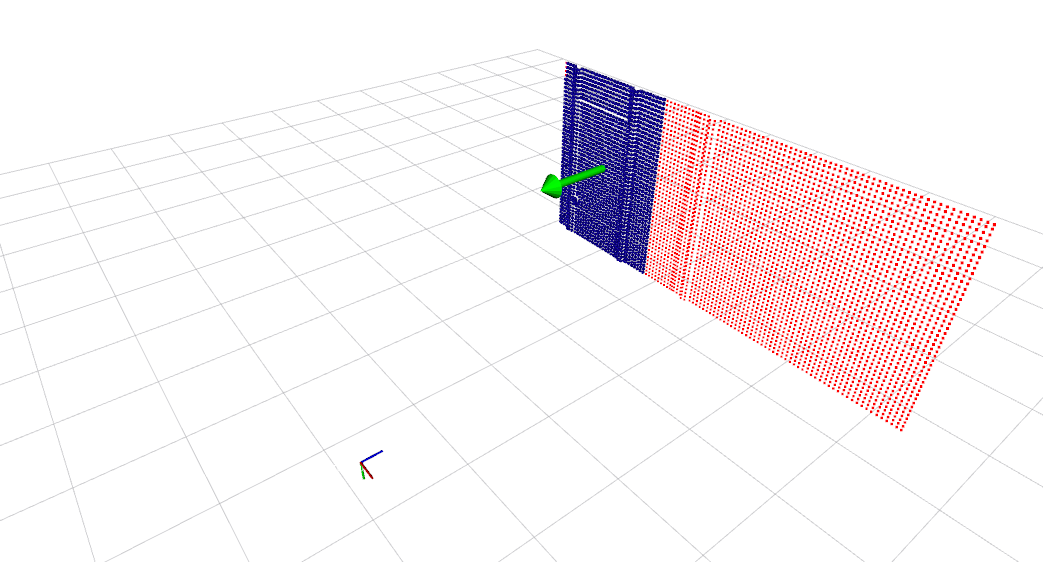
\includegraphics[width=0.5\linewidth]{images/pcl/Selection_064} &
  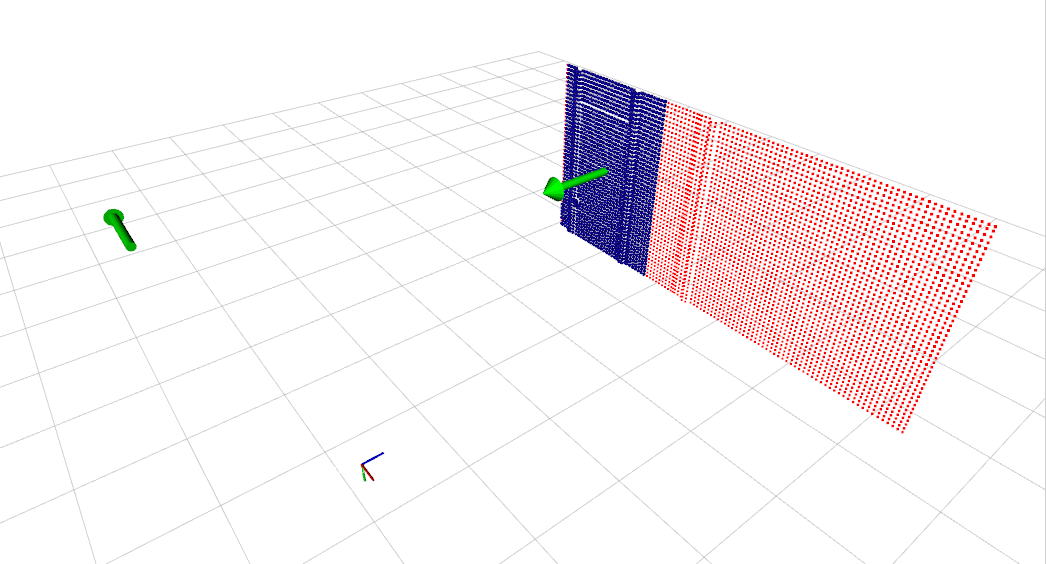
\includegraphics[width=0.5\linewidth]{images/pcl/Selection_065} \\
  (5) & (6)
\end{tabular}

(1) Nuage de points initial. (2) Downsampling du nuage. (3) Filtrage du sol par seuillage de la coordonnée $z$. (4) Sélection de un tiers du nuage vers l'avant du robot. (5) Calcul de la normale par ACP. (6) Calcul de la nouvelle pose objectif en prenant une longueur de pas dans la direction obtenue par le produit vectoriel entre la normale et l'axe $z$ du robot.

\Annexe{Machine à états pour l'inspection d'éoliennes}
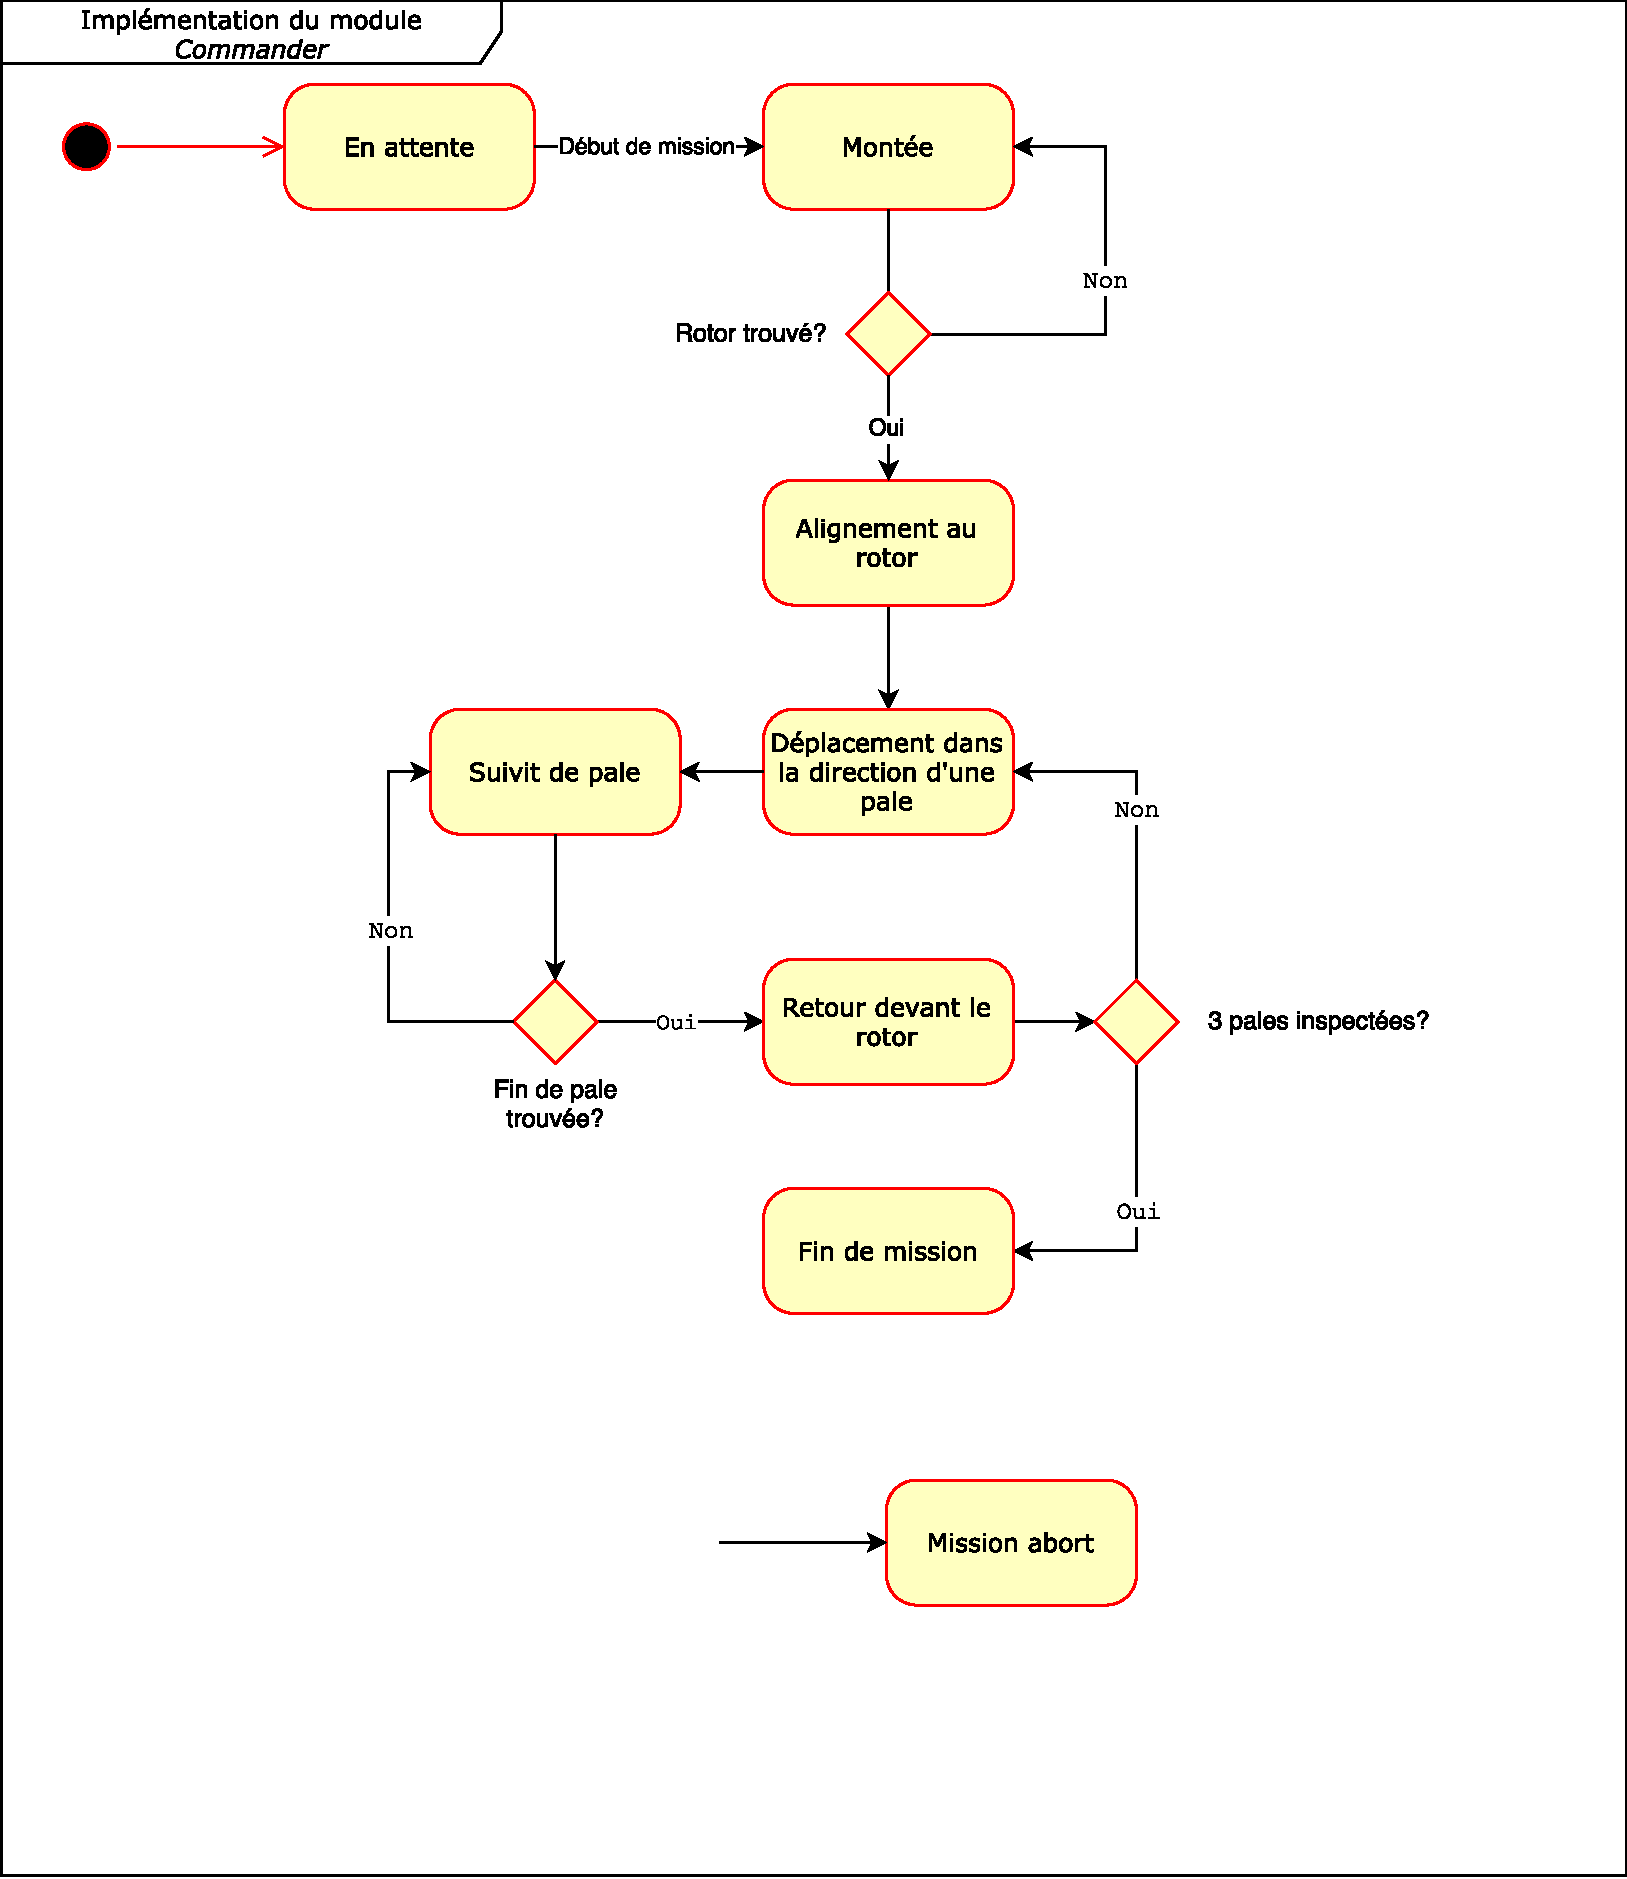
\includegraphics[width=\linewidth]{images/state_machine.pdf}
\label{annexe:state_machine}

%%  Toutes les annexes doivent être inclues dans ce document
%%  les unes à la suite des autres.
% \Annexe{DÉMO}
% Texte de l'annexe A\@. Remarquez que la phrase précédente se termine
% par une lettre majuscule suivie d'un point. On indique explicitement
% cette situation à \LaTeX{} afin que ce dernier ajuste correctement
% l'espacement entre le point final de la phrase et le début de la
% phrase suivante.


%\begin{landscape}
%\Annexe{ENCORE UNE ANNEXE}
%Texte de l'annexe B\@ en mode «landscape».
%\end{landscape}
%
%\Annexe{UNE DERNIÈRE ANNEXE}
%Texte de l'annexe C\@.
